\documentclass{article}

\usepackage[utf8]{inputenc}
\usepackage{polski}
\usepackage{titlesec}
\usepackage{graphicx}
\graphicspath{ {images/} }

\title{Generator ruchu Google Analytics \\ Iteracja I architektura systemu}
\author{Bartłomiej Dalak \and Bartłomiej Karwowski \and Bartosz Gromek \and Tomasz Kanas}

\begin{document}
\maketitle

\section{Wstęp}

Dokument architektury systemu ma na celu przedstawienie wizji architektury. Opisana architektura może ulec zmianom w fazie implementacji.

\section{Opis elementów architektury}

\subsection{Aplikacja}

Aplikacją w naszym przypadku będzie skrypt "generate\_ga\_traffic.py", generujący ruch według podanych przez użytkownika wartości. Będzie on uruchamiany przez konsolę.

\subsubsection{Język}

Wykorzystany zostanie Python w wersji 3.6.

\subsubsection{Użyte biblioteki}

\begin{itemize}
\item request: wysyłanie zapytań do GA
\item threading: tworzenie wątku działającego w tle(daemon)
\end{itemize}

\section{Schemat działania}

\subsection{Wygenerowanie danych}
Po otrzymaniu danych od użytkownika zostaną wygenerowane dane za pomocą generate\_data\_api.

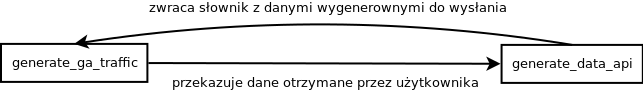
\includegraphics[scale=0.5]{generate}

\subsection{Wysyłanie danych}
Będziemy wysyłać dane używając napisanego przez nas API: send\_requests\_api.

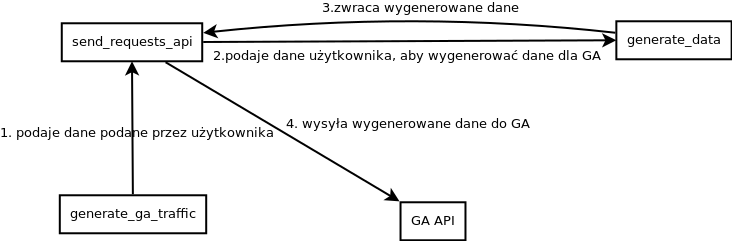
\includegraphics[scale=0.5]{connection_ga}

\end{document}
